\documentclass{article}
% For math environments
\usepackage{amsmath, amsfonts}
% For links
\usepackage[colorlinks=true,
    linkcolor = blue,
    urlcolor  = blue,
    citecolor = blue,
    anchorcolor = blue]{hyperref}
% Put space between paragraphs
\usepackage{parskip}
% For figures
\usepackage{tikz}
% Set the margins to not be ridiculous
\usepackage[margin=0.75in]{geometry}
% For multiple columns
\usepackage{multicol}
% For controlling enum/itemize spacing and indentation
\usepackage{enumitem}
% More math symbols
\usepackage{amssymb}
% To change enumerate labels

% For tikz plots
\usepackage{pgfplots}
% This isn't needed but avoids a compiler warning
\pgfplotsset{compat=1.16}

% Allow multi-line equations to be broken across pages
\allowdisplaybreaks

% Use @ as a letter
\makeatletter

% Scale down all tikz coordinates while maintaining font size
\tikzset{every picture/.style={scale=0.45, every picture/.style={}}}


% Macros
% Monospace code
\def\code#1{\texttt{#1}}

% Greek letters
\def\a{\alpha}
\def\b{\beta}
\def\g{\gamma}
\def\d{\delta}
\def\D{\Delta}

% Commands that make life easier
\newcommand\gath[1]{\begin{gather} #1 \end{gather}}
\newcommand\ali[1]{\begin{align} #1 \end{align}}
\newcommand\parens[1]{\left( #1 \right)}
\newcommand\squares[1]{\left[ #1 \right]}
\newcommand\braces[1]{\left\{ #1 \right\}}
\newcommand\angles[1]{\left\langle #1 \right\rangle}
\newcommand\deriv[2]{\frac{d #1}{d #2}}
\newcommand\abs[1]{\left| #1 \right|}
\newcommand\floor[1]{\left\lfloor #1 \right\rfloor}
\DeclareMathOperator{\lcm}{lcm}
\def\non{\nonumber \\}

% Multiline equation space
\def\mlesp{\hspace{1.2cm}}

% For grid diagrams
\newcommand\gridbox[3]{\draw (#1,#2) rectangle (#1+1,#2+1) node[pos=.5] {#3};}
\newcommand\gridboxh[3]{\draw[fill=red!20] (#1,#2) rectangle (#1+1,#2+1) node[pos=.5] {#3};}
\newcommand\gridboxb[3]{\draw[fill=black] (#1,#2) rectangle (#1+1,#2+1) node[pos=.5] {#3};}
\newcommand\gridsym[3]{\node at (#1+0.5,#2+0.5) {$#3$};}
\newcommand\gridblank[2]{\filldraw[draw=gray, color=gray] (#1,#2) rectangle (#1+1,#2+1);}
\newcommand\gridcirc[2]{\draw (#1 + 0.5,#2 + 0.5) circle (0.25);}
\newcommand\cwlab[3]{
  \def\dd{0.15}
  \draw (#1 + \dd - 0.03, #2 + 1 - \dd) node {\scriptsize #3};
}

\def\bbw{3.5}
\def\bbh{2}
\newcommand\bigbox[3]{\draw (#1*\bbw,#2*\bbh) rectangle (#1*\bbw+\bbw,#2*\bbh+\bbh) node[pos=.5] {#3};}
\newcommand\bbtextr[3]{\node[right] at (#1*\bbw,#2*\bbh+0.5*\bbh) {#3};}
\newcommand\bbtextb[3]{\node[align=center] at (#1*\bbw+0.5*\bbw,#2*\bbh+0.5*\bbh) {#3};}

% Box puzzle stock answer
\newcommand\boxans[1]{
  Logic was used to deduce the solution:

  #1

  This was verified using Python as well as shown to be unique with a brute force approach.
}

% Multiple numbers
\newcommand\mn[1]{$#1$'s}

% Commands for problems
\newcommand\problem[4]{
  \section*{#1}

  Question: #3
  
  Answer: #2
  
  Explanation: #4
}
\newcommand\aproblem[4]{\problem{Dec #1}{#2}{#3}{#4}}
\newcommand\cproblem[4]{\problem{Problem #1}{#2}{#3}{#4}}

\def\advent@xxiv@i{
  Eve writes down five different positive integers.
  The sum of her integers is $16$. What is the product of her integers?
}

\def\advent@xxiv@ii{
  $14$ is the smallest even number that cannot be obtained by rolling two $6$-sided dice and finding the product of the numbers rolled.

  What is the smallest even number that cannot be obtained by rolling one hundred $100$-sided dice and finding the product of the numbers rolled?
}

\def\advent@xxiv@iii{
  There are $5$ ways to write $5$ as the sum of positive odd numbers:
  \begin{itemize}
    \item $1 + 1 + 1 + 1 + 1$
    \item $1 + 1 + 3$
    \item $3 + 1 + 1$
    \item $1 + 3 + 1$
    \item $5$
  \end{itemize}

  How many ways are there to write $14$ as the sum of positive odd numbers?
}

\def\advent@xxiv@iv{
  The geometric mean of a set of $n$ numbers is computed by mulitplying all the numbers together, then taking the $n$th root.
  The factors of $9$ are $1$, $3$, and $9$.
  The geometric mean of these factors is
  \gath{
    \sqrt[3]{1 \times 3 \times 9} = \sqrt[3]{27} = 3
  }
  What is the smallest number where the geometric mean of its factors is $13$?
}

\def\advent@xxiv@v{
  The sum of $11$ consecutive integers is $2024$.
  What is the smallest of the $11$ integers?
}

\def\advent@xxiv@vi{Put the digits 1 to 9 (using each digit exactly once) in the boxes so that the sums are correct. The sums should be read left to right and top to bottom ignoring the usual order of operations. For example, 4+3×2 is 14, not 10. Today's number is the product of the numbers in the red boxes.
  The number $n$ has $55$ digits.
  All of its digits are $9$.
  What is the sum of the digits of $n^3$?
}

\def\advent@xxiv@vii{
  What is the obtuse angle in degrees between the minute and hour hands of a clock at 08:22?
}

\def\advent@xxiv@viii{
  It is possible to arrange $4$ points on a plane and draw non-intersecting lines between them to form $3$ non-overlapping triangles:

  \begin{center}
    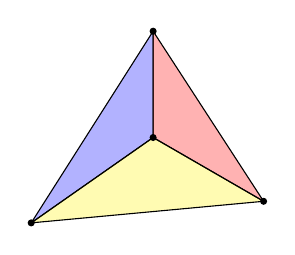
\begin{tikzpicture}
      \def\ds{3}
      \def\pa{(0: 0)}
      \def\pb{(90: \ds)}
      \def\pc{(215: 1.4*\ds)}
      \def\pd{(-30: 1.2*\ds)}

      \def\bcr{3}
      \def\scr{0.55*\bcr}
      \def\sca{34}
      \def\mcr{0.7*\bcr}
      \def\mca{142}
      \def\pr{0.1}

      % Triangles
      \draw[fill=blue,fill opacity=0.3] \pa -- \pb -- \pc -- cycle;
      \draw[fill=red,fill opacity=0.3] \pa -- \pb -- \pd -- cycle;
      \draw[fill=yellow,fill opacity=0.3] \pa -- \pd -- \pc -- cycle;

      % Points
      \fill \pa circle (\pr);
      \fill \pb circle (\pr);
      \fill \pc circle (\pr);
      \fill \pd circle (\pr);
    \end{tikzpicture}
  \end{center}

  It is not possible to make more than $3$ triangles with $4$ points.

  What is the maximum number of non-overlapping triangles that can be made by arranging $290$ points on a plane and drawing non-intersecting lines between them?
}

\def\advent@xxiv@ix{
  Put the digits $1$ to $9$ (using each digit exactly once) in the boxes so that the sums are correct.
  The sums should be read left to right and top to bottom ignoring the usual order of operations.
  For example, $4 + 3 \times 2$ is $14$, not $10$.
  Today's number is the product of the numbers in the red boxes.

  \grid@advent@xxiv@ix{}{}{}{}{}{}{}{}{}
}

\def\advent@xxiv@x{
  A number is a palindrome if it's the same when its digits are written in reverse order.

  What is the sum of all the numbers between $10$ and $100$ that are palindromes?
}

\def\advent@xxiv@xi{
  There are $6$ sets of integers between $1$ and $5$ (inclusive) that contain an odd number of numbers whose median value is $3$:

  \begin{itemize}
    \item $\braces{3}$
    \item $\braces{1,3,4}$
    \item $\braces{2,3,4}$
    \item $\braces{1,3,5}$
    \item $\braces{2,3,5}$
    \item $\braces{1,2,3,4,5}$
  \end{itemize}

  How many sets of integers between $1$ and $11$ (inclusive) are there that contain an odd number of numbers whose median value is $5$?
}

\def\advent@xxiv@xii{
  Holly picks a three-digit number.
  She then makes a two-digit number by removing one of the digits.
  The sum of her two numbers is $309$.
  What was Holly's original three-digit number?
}

\def\advent@xxiv@xiii{
  Today's number is given in this crossnumber.
  No number in the completed grid starts with $0$.

  \begin{multicols}{2}
    \crossnumstd{}{}{}{}{}{}{}{}{}

    \vfill\null
    \columnbreak

    \begin{center}
      \textbf{Across}

      \begin{tabular}{clc}
        \textbf{1} & Today's number.  & (\textbf{3}) \\
        \textbf{4} & Two times 5A.    & (\textbf{3}) \\
        \textbf{5} & A multiple of 1. & (\textbf{3})
      \end{tabular}

      \textbf{Down}

      \begin{tabular}{clc}
        \textbf{1} & Sum of digits is 15. & (\textbf{3}) \\
        \textbf{2} & Sum of digits is 19. & (\textbf{3}) \\
        \textbf{3} & Three times 5A.      & (\textbf{3})
      \end{tabular}
    \end{center}
  \end{multicols}
}

\def\advent@xxiv@xiv{
  $15^3$ is $3375$.
  The last $3$ digits of $15^3$ are $375$.

  What are the last $3$ digits of $15^{1234567890}$?
}

\def\advent@xxiv@xv{
  The number $2268$ is equal to the product of a square number (whose last digit is not $0$) and the same square number with its digits reversed: $36 \times 63$.

  What is the smallest three-digit number that is equal to the product of a square number (whose last digit is not $0$) and the same square number with its digits reversed?
}

\def\advent@xxiv@xvi{
  Put the digits $1$ to $9$ (using each digit exactly once) in the boxes so that the sums are correct.
  The sums should be read left to right and top to bottom ignoring the usual order of operations.
  For example, $4 + 3 \times 2$ is $14$, not $10$.
  Today's number is the product of the numbers in the red boxes.

  \grid@advent@xxiv@xvi{}{}{}{}{}{}{}{}{}
}

\def\advent@xxiv@xvii{
  The number $40$ has $8$ factors: $1$, $2$, $4$, $5$, $8$, $10$, $20$, and $40$.

  How many factors does the number $2^{26} \times 5 \times 7^5 \times 11^2$ have?
}

\def\advent@xxiv@xviii{
  TODO
}

\def\card@xxiv@i{
  What is the largest number you can make by using the digits $1$ to $4$ to make two $2$-digit numbers, then mutiplying the two numbers together?
}

\def\card@xxiv@ii{
  What is the largest number you can make by using the digits $0$ to $9$ to make a $2$-digit number and an $8$-digit number, then mutiplying the two numbers together?
}

\def\card@xxiv@iii{
  The expansion of $(2x+3)^2$ is $4x^2 + 12x + 9$.
  The sum of the coefficients of $4x^2 + 12x + 9$ is $25$.
  What is the sum of the coefficients of the expansion of $(30x + 5)^2$?
}

\def\card@xxiv@iv{
  What is the sum of the coefficients of the expansion of $(2x+1)^{11}$?
}

\def\card@xxiv@v{
  What is the geometric mean of all the factors of $41306329$?
}

\def\card@xxiv@vi{
  What is the largest number for which the geometric mean of all its factors is $92$?
}

\def\card@xxiv@vii{
  What is the sum of all the factors of $7^4$?
}

\def\card@xxiv@viii{
  How many numbers between $1$ and $28988500000$ have an odd number of factors?
}

\def\card@xxiv@ix{
  Eve found the total of the $365$ consecutive integers starting at $500$ and the total of the next $365$ consecutive integers, then subtracted the smaller total from the larger total.
  What was her result?
}

\def\card@xxiv@x{
  Eve found the total of the $n$ consecutive integers starting at a number and the total of the next $n$ consecutive integers, then subtracted the smaller total from the larger total.
  Her result was $22344529$.
  What is the largest possible value of $n$ that she could have used?
}

\input{boxes}

\begin{document}

\title{MS Scroggs Advent Calendar 2019 Answers}
\author{Dan Whitman}
\date{}

\maketitle

Answers: \href{https://www.mscroggs.co.uk/puzzles/advent2019}{https://www.mscroggs.co.uk/puzzles/advent2019}

\aproblem{1}{301}{\advent@xix@i}{
  Each of the digits will be one 100 times since there are 100 combinations of the other two digits.
  Thus the total number of ones written in the numbers 1 to 999 are
  $$
  100 + 100 + 100 = 300 \,.
  $$
  Then of course 1000 only has one 1 so that the final answer is $300 + 1 = 301$.

  This answer was verified using Python.
}

\aproblem{2}{203}{\advent@xix@ii}{
  A valid triangle can only be formed when the sum of two sides is greater than the third side, so we really only need to check that the two smallest sides sum to greater than the third, largest side.
  If the sum is equal to the third side the sticks must “lay on top of each other,'' which we are told is not a valid triangle.
  Furthermore, given three valid sides, the triangle is unique up to reflection and rotation.
  A Python script was written to count the number of valid triangles for this set of sides, i.e. where the two shortest sides sum to greater than the longest side.
}

\aproblem{3}{432}{\advent@xix@iii}{
  \boxans{\gridsol@advent@xix@iii}
}

\newcommand\tilerect[2]{\draw[color=red!75,line width=2] (#1) rectangle (#2);}
\newcommand\tilefig[2]{
  \begin{tikzpicture}
    \draw (0,0) grid (#1);
    #2
  \end{tikzpicture}
  \qquad
}
\def\contd{
  \draw (0,0) -- (0,-0.5);
  \draw (1,0) -- (1,-0.5);
  \draw (2,0) -- (2,-0.5);
  \node[align=center] at (1,-0.7) {$\cdots$};
}

\aproblem{4}{341}{\advent@xix@iv}{
  There are clearly exactly 3 ways to tile a $2 \times 2$ grid:
  \begin{center}
    \tilefig{2,2}{
      \tilerect{0,0}{2,2}
    }
    \tilefig{2,2}{
      \tilerect{0,0}{1,2}
      \tilerect{1,0}{2,2}
    }
    \tilefig{2,2}{
      \tilerect{0,0}{2,1}
      \tilerect{0,1}{2,2}
    }
  \end{center}
  Let $s_n$ denote the the number of ways to tile an $n \times 2$ grid.
  Then we know that $s_1 = 1$ and $s_2 = 3$.
  We can generally determine $s_n$ using an approach similar to strong induction.
  If we know $s_k$ for $k < n$, then there are 3 ways to cover the first row of an $n \times 2$ grid:
  \begin{center}
    \tilefig{2,3}{
      \contd
      \tilerect{0,1}{2,3}
    }
    \tilefig{2,3}{
      \contd
      \tilerect{0,1}{1,3}
      \tilerect{1,1}{2,3}
    }
    \tilefig{2,3}{
      \contd
      \tilerect{0,2}{2,3}
    }
  \end{center}
  For each of the first two of these ways we must cover the remaining $(n-2) \times 2$ grid and there are of course $s_{n-2}$ ways to do this.
  For the third we must cover the remaining $(n-1) \times 2$ grid, of which there are $s_{n-1}$ ways.
  Therefore the total number of ways to cover an $n \times 2$ grid is
  $$
  s_n = s_{n-2} + s_{n-2} + s_{n-1} = s_{n-1} + 2s_{n-2} \,.
  $$
  This forms a sequence not unlike the Fibonacci sequence.
  The first ten elements of the sequence are:
  \begin{center}
    \begin{tabular}{c|cccccccccc}
      $n$ & 1 & 2 & 3 & 4 & 5 & 6 & 7 & 8 & 9 & 10 \\
      \hline
      $s_n$ & 1 & 3 & 5 & 11 & 21 & 43 & 85 & 171 & 341 & 683
    \end{tabular}
  \end{center}
  Thus the answer is $s_9 = 341$.
  This sequence was confirmed to be correct on OEIS, and is the Jacobsthal sequence.
  The notes for this sequence mention it being the number of ways to tile a $n \times 2$ grid using the specified dominoes.
}

\aproblem{5}{364}{\advent@xix@v}{
  The 28 points on the circle are spaced $\Delta \theta = 360/28 = 90/7 \approx 12.86$ degrees apart.
  The radius of the circle is of course irrelevant here so we may as well use the unit circle.
  We number the points $p_n$ for $0 \leq n < 28$ and we can place $p_0$ at $(1,0)$ and count counterclockwise so that we have the following example points that divide the circle into quarters:
  \begin{center}
    \begin{tabular}{c|c}
      $n$ & $p_n$ \\
      \hline
      0 & $(1,0)$ \\
      7 & $(0,1)$ \\
      14 & $(-1,0)$ \\
      21 & $(0,-1)$
    \end{tabular}
  \end{center}
  Now, given one of the 28 points as a base, say $p = p_{14} = (-1,0)$, we can choose any other 2 distinct points to create a triangle.
  However, clearly this triangle will be isosceles with the two equal sides emanating from $p$ only when a point on the top half is chosen along with its mirror point on the bottom half when reflected over the $x$-axis.
  As there are 13 of these point-pairs, 13 of the triangles emanating from $p$ will be isosceles.
  Since this is done for each of the 28 points, there can be at most $13 \cdot 28 = 364$ isosceles triangles.

  The question arises as to whether we are counting some isosceles triangles more than once though.
  The only way this could be the case is if we have equilateral triangles wherein more than one point acts as the base from which the equal sides emanate.
  However, a third of the circle or $360/3 = 120$ degrees is not an integer multiple of our $\Delta \theta$, which means that no 3 of our 28 points can be evenly spaced around the circle.
  Because of this there can be no equilateral triangles since sides of any triangle is the chord length $2\sin(\theta/2)$, where $\theta$ is the positive angle between the points.
  From this it follows that we have exactly $364$ isosceles triangles.

  This answer was confirmed with a brute force Python program.
}

\aproblem{6}{221}{\advent@xix@vi}{
  Suppose that Noel has $N$ grandchildren, and let $t_n$ be the total number of pounds given to all his grandchildren on the year that the \emph{youngest} is $n$ years old (and therefore gets $n$ pounds).
  As the children were all born on consecutive years, the total they are given on year $n$ is
  $$
  t_n = \sum_{i=0}^{N-1} (n+i) = \sum_{i=0}^{N-1} n + \sum_{i=0}^{N-1} i = Nn + \sum_{i=1}^{N-1} i = Nn + \frac{N(N-1)}{2} = \frac{N(N + 2n - 1)}{2} \,,
  $$
  noting that this is monotonically increasing in both $N$ and $n$.
  Python was used to evaluate $t_n$ for all combinations of $N,n \in \{1, 2, \ldots, 20\}$.
  It showed that the only combination where $t_n = 208$ is for $N = 13$ and $n = 10$.
  Note that, because of the monotonicity of $t_n$ in both $N$ and $n$, $t_n > 208$ for all $N > 13$ and $n > 10$ so that we a guaranteed not to have another combination where $t_n = 208$.
  Hence the total number of pounds his grandchildren get the next year is $t_{n+1} = t_n + N = 221$.
}

\aproblem{7}{243}{\advent@xix@vii}{
  In general, the binomial theorem states that
  $$
  (x+y)^n = \sum_{k=0}^n \binom{n}{k} x^{n-k} y^k \,,
  $$
  where of course $\binom{n}{k}$ are the binomial coefficients.
  Hence, for the example we have
  $$
  (x+1)^5 = (1+x)^5 = \sum_{k=0}^5 \binom{5}{k} 1^{5-k} x^k = \sum_{k=0}^5 \binom{5}{k} x^k
  $$
  so that the sum of coefficients is simply
  $$
  \sum_{k=0}^5 \binom{5}{k} = 32
  $$
  as confirmed using Python.
  For the main problem we then have
  $$
  (2x+1)^5 = (1+2x)^5 = \sum_{k=0}^5 \binom{5}{k} 1^{5-k} (2x)^k = \sum_{k=0}^5 \binom{5}{k} 2^k x^k \,,
  $$
  and thus the sum of the coefficients is
  $$
  \sum_{k=0}^5 \binom{5}{k} 2^k = 243
  $$
  as calculated in Python.
  This answer was also verified by expanding $(2x+1)^5$ in Wolfram Alpha and summing the $6$ coefficients manually.
}

\aproblem{8}{270}{\advent@xix@viii}{
  Generally we want the highest digits in the tens places and the lowest digits in the ones places, noting again that all five numbers must be even.
  However, it does not matter which ones digit goes with which number.
  For example
  \begin{align*}
    10 + 32 + 54 + 76 + 98 &= (10 + 0) + (30 + 2) + (50 + 4) + (70 + 6) + (90 + 8) \\
    &= (10 + 8) + (30 + 6) + (50 + 4) + (70 + 2) + (90 + 0) \\
    &= 18 + 36 + 54 + 72 + 90 \\
    &= 270 \,,
  \end{align*}
  which is in fact the largest possible sum.
  This was verified in Python using a brute force method to check every possible permutation of digits into 5 two-digit numbers.
}

\aproblem{9}{523}{\advent@xix@ix}{
  \boxans{\grid@advent@xix@ix{5}{7}{1}{2}{8}{4}{3}{9}{6}}
}

\aproblem{10}{256}{\advent@xix@x}{
  Define $g(x) = 8x - 8 - x^2$ and $h(x) = x^2$, which are of course both parabolas.
  Then we know that $g(x) \leq f(x) \leq h(x)$ for all real $x$.
  A plot of $g$ and $h$ are shown below:
  
  \newcommand\doplot[1]{
    \begin{center}
      \begin{tikzpicture}[scale=1.8]
        \begin{axis}[
            axis lines=middle,
            xmin=-5, xmax=5,
            ymin=-70, ymax=30,
            samples=100,
          ]
          \addplot[
            blue,
            thick,
            domain=-5:5,
          ]
          (x, x^2);
          \node [above right] at (axis cs:-4,16) {$h$};
          \addplot[
            red,
            thick,
            domain=-5:5,
          ]
          (x, 8*x - 8 - x^2);
          \node [below right] at (axis cs:-4,-56) {$g$};
          #1
        \end{axis}
      \end{tikzpicture}
    \end{center}
  }
  \doplot{}
  
  We notice that they appear to touch at a single point and that there seems to be just enough space for a single line to squeeze through.
  To see whether they touch at a single point we set
  \begin{gather*}
    g(x) = h(x) \\
    8x - 8 - x^2 = x^2 \\
    8x - 8 = 2x^2 \\
    4x - 4 = x^2 \\
    x^2 - 4x + 4 = 0 \\
    (x - 2)^2 = 0 \,.
  \end{gather*}
  Therefore they intersect at the single point $(2, g(x)) = (2, h(2)) = (2, 4)$.
  Hence we also must have $4 = g(2) \leq f(2) \leq h(2) = 4$ so that $f(2) = 4$.
  We also have that $g'(x) = 8 - 2x$ and $h'(x) = 2x$ so that $g'(2) = h'(2) = 4$.
  Indeed it must be that $g$ and $h$ have the same slope at their intersection point in order for a line to pass in between them at all points.

  So the line we seek is the tangent line of both parabolas at their intersection point.
  That is a line with slope $a = 4$ and passes through the point $(2,4)$.
  Solving $4 = f(2) = 4 \cdot 2 + b$ for $b$ results in our line $f(x) = 4x-4$.
  A plot of the parabolas along with this line is shown below:

  \doplot{
    \addplot[
      black,
      thick,
      domain=-5:5,
    ]
    (x, 4*x - 4);
    \node [below right] at (axis cs:-4,-20) {$f$};
  }
  
  This confirms that $f$ is the correct line.
  Therefore the answer is $f(65) = 256$.
}

\aproblem{11}{192}{\advent@xix@xi}{
  \boxans{\gridsol@advent@xix@xi}
}

\aproblem{12}{643}{\advent@xix@xii}{
  There are $T = 650 \cdot 99 = 64350$ total voters.
  Half of these voted for the Rum party, which is of course $T/2$, noting that this is an integer since $T$ is even.
  Now, the Rum party must get exactly $50$ votes in a district to win the MAP and ``spend'' the minimum number of its $T/2$ voters since this is a minimal majority for $99$ voters.
  Therefore the maximal number of MAPs that the Rum party can win is $\lfloor T/2/50 \rfloor = \lfloor T/100 \rfloor = 643$, noting that the floor is necessary since a district with less than $50$ votes will not be won.
}

\aproblem{13}{211}{\advent@xix@xiii}{
  \boxans{\grid@advent@xix@xiii{2}{1}{5}{2}{1}{2}{1}{1}{9}}
}

\aproblem{14}{112}{\advent@xix@xiv}{
  This was solved with a simple Python script that sums the digits and counts how many add to $14$.
}

\aproblem{15}{203}{\advent@xix@xv}{
  This was solved using Python, which was challenging to implement.
  It was noticed that both $30 = 2 \cdot 3 \cdot 5$ and $30030 = 2 \cdot 3 \cdot 5 \cdot 7 \cdot 11 \cdot 13$ factor into unique prime factors with no repeated factors.
  If $f(n)$ denotes the number of ways to multiply a number with $n$ unique prime factors, then this forms the following sequence, which was determined by experimentation with the Python script:
  \begin{center}
    \begin{tabular}{c|c}
      $n$ & $f(n)$ \\
      \hline
      1 & 1 \\
      2 & 2 \\
      3 & 5 \\
      4 & 15 \\
      5 & 52 \\
      6 & 203 \\
      7 & 877
    \end{tabular}
  \end{center}
  Looking it up on OEIS, this is the Bell sequence, given by the recurrence relation
  $$
  f(n) = \sum_{k=0}^n \binom{n}{k} f(k) \,.
  $$
  I struggled to deduce this relation but failed.
}

\aproblem{16}{921}{\advent@xix@xvi}{
  Tried to deduce the grid solution, but eventually got stuck and would have had to guess.
  As such, this was just solved using a brute force search in Python:

  \grid@advent@xix@xvi{9}{6}{5}{2}{8}{3}{1}{7}{4}
}

\aproblem{17}{193}{\advent@xix@xvii}{
  Let $x$ be Eve's original number with the digits $d_2 d_1 d_0$, and let $y$ be the second, reversed number, which would then have digits $d_0 d_1 d_2$.
  Now, we know that $d_2 > 0$ since $x$ is a three-digit number.
  We are also told that $y > x$, from which it follows that $d_2 \neq d_0$ since otherwise it would be that $x = y$.
  Moreover we must have $d_0 > d_2$ since $y > x$.
  Lastly, we know that
  \begin{gather*}
    x + y = 584 \\
    (100 d_2 + 10 d_1 + d_0) + (100 d_0 + 10 d_1 + d_2) = 584 \\
    100(d_2 + d_0) + 20 d_1 + (d_2 + d_0) = 584 \\
    10 [ 10(d_2 + d_0) + 2d_1] + (d_2 + d_0) = 584 \,.
  \end{gather*}
  The first term is a multiple of $10$ and so the least significant digit of this number is zero.
  Hence it must be that the least significant digit of $d_2 + d_0$ is $4$, and so either $d_2 + d_0 = 4$ or $d_2 + d_0 = 14$.
  Since $d_0 > d_2 > 0$, it cannot be that $d_2 = d_0 = 2$ or that $d_2 = d_0 = 7$.
  Likewise, it cannot be that $(d_2, d_0) = (0, 4)$.
  So we have the following remaining possibilities: $(d_2, d_0) = (1,3)$, $(d_2,d_0) = (6,8)$, or $(d_2,d_0) = (5,9)$.

  Now we momentarily digress and solve for $d_1$ in the case when $d_2$ and $d_0$ are known.
  We have
  \begin{gather*}
    100(d_2 + d_0) + 20 d_1 + (d_2 + d_0) = 584 \\
    101(d_2 + d_0) + 20 d_1 = 584 \\
    d_1 = \frac{584 - 101(d_2 + d_0)}{20} \,.
  \end{gather*}
  The results of this when we plug in our possible values of $d_2$ and $d_0$ are summarized below:
  \begin{center}
    \begin{tabular}{cc|c}
      $d_2$ & $d_0$ & $d_1$ \\
      \hline
      1 & 3 & 9 \\
      6 & 8 & -83/2 \\
      5 & 9 & -83/2
    \end{tabular}
  \end{center}
  Of course of these only $9$ is a reasonable value for a digit!
  So it must be that $(d_2, d_1, d_0) = (1, 9, 3)$ so that $x = 193$ and $y = 391$.

  This answer was confirmed with python as well as ensuring that it is unique using brute force to check every possible three-digit number.
}

\aproblem{18}{791}{\advent@xix@xviii}{
  This is of course a single-heap game of \href{https://en.wikipedia.org/wiki/Nim}{Nim}.
  In general, if each player can take anywhere from $1$ and $k$ (inclusive) items, then the perfect-play strategy is to always take the right number of items so that the number left for the other player is is congruent to zero modulo $k+1$.
  The translates to always removing $N \mod k+1$ from the pile of $N$ items on your turn, assuming this possible.
  This is only impossible when $N \equiv 0 \mod k+1$ since you cannot remove $0$ items or $k+1$ items to make it zero modulo $k+1$ again.
  In the case your opponent will always win if they play perfectly.
  
  In our case $k = 900$ and we start with $N = 1000000$ pounds, so we must remove $n = 791$ pounds since $N - n \equiv 0 \mod k+1$, that is $999209 \equiv 0 \mod 901$.
}

\aproblem{19}{112}{\advent@xix@xix}{
  First we note that for a square with side length $s$, the diagonal radius, i.e. the length from center of the square to to any of the corners, is $d = s/\sqrt{2}$.
  Similarly the diagonal, i.e. the length from a corner to the opposite corner, is $\sqrt{2} s = 2d$.
  Both of these are trivial to show using the Pythagorean theorem.
  
  Now let $A_b$ and $s_b$ denote the area and side length, respectively, of the blue square so that of course $A_b = s_b^2 = 14$.
  Also let $R$ denote the radius of the large circle and $S$ denote the side of the large enclosing square so that we have $R = S/2$.
  We then have that the diagonal radius of the largest square is
  \begin{gather*}
    \frac{S}{\sqrt{2}} = R + \sqrt{2}s_b = \frac{S}{2} + \sqrt{2}s_b \\
    \frac{S}{\sqrt{2}} - \frac{S}{2} = \sqrt{2}s_b \\
    S = \frac{\sqrt{2}s_b}{\frac{1}{\sqrt{2}} - \frac{1}{2}} \\
    S = \frac{4 s_b}{2 - \sqrt{2}} \,.
  \end{gather*}
  Now let $r$ be the radius of the smaller circles, $A_r$ be the area of the red square, and $s_r$ be the side length of the red square.
  Then of course $A_r = s_r^2$, but we also clearly have that $s_r = 2r$ and the diagonal radius of the red square is $d_r = s_r / \sqrt{2} = 2r / \sqrt{2} = \sqrt{2}r$.
  We also have $d_r + r = R$, and thus
  \begin{gather*}
  \sqrt{2}r + r = R \\
  r = \frac{R}{\sqrt{2} + 1}
  \end{gather*}
  Putting this all together, we have
  \begin{align*}
    A_r &= s_r^2 = (2r)^2 = 4r^2 = \frac{4R^2}{(\sqrt{2}+1)^2} = \frac{4}{(\sqrt{2}+1)^2} \left(\frac{S}{2} \right)^2 \\
    &= \frac{S^2}{(\sqrt{2}+1)^2} = \frac{1}{(\sqrt{2}+1)^2} \left(\frac{4 s_b}{2 - \sqrt{2}}\right)^2 \\
    &= \frac{16s_b^2}{[(\sqrt{2}+1)(2 - \sqrt{2})]^2} = \frac{16 A_b}{(2\sqrt{2} - 2 + 2 - \sqrt{2})^2} \\
    &= \frac{16 A_b}{(\sqrt{2})^2} = \frac{16 A_b}{2} = 8 A_b \,.
  \end{align*}
  Therefore the answer is $A_r = 8 A_b = 8 \cdot 14 = 112$, which was verified using Python in a somewhat rudimentary way.
}

\aproblem{20}{858}{\advent@xix@xx}{
  This can be reasoned through by looking at the unique prime decomposition of each of the numbers on the cards:
  \begin{align*}
    2 &= 2 & 7 &= 7 & 11 &= 11 \\
    3 &= 3 & 8 &= 2^3 & 12 &= 2^2 \cdot 3 \\
    4 &= 2^2 & 9 &= 3^2 & 13 &= 13 \\
    5 &= 5 & 10 &= 2 \cdot 5 & 14 &= 2 \cdot 7 \\
    6 &= 2 \cdot 3
  \end{align*}
  Now, in order for the two hands of five numbers to have the same product, they must each contain the same prime factors.
  Hence, if a prime factor appears in one of these hands, the same factor must also appear in the other hand in an equal power.
  We first notice that the prime factors $11$ and $13$ both only appear in a single card so that these two cards must be in the set of cards left on the table since, if they were in one of the hands, the other hand could not contain these factors to cancel out.

  We also notice that the $5$ card must be in one hand and the $10$ card must be in the other as these are the only the two cards containing $5$ as a prime factor.
  This follows since, if either of these were left on the table, the other must be in one the hands (since we know the other two cards on the table) with no other factor $5$ in the other hand to cancel it out.
  For the same reason $7$ must be in one hand and $14$ in the other since these are the only cards containing $7$ as a prime factor.

  Of the remaining cards whose positions are unknown, i.e. $\{2,3,4,6,8,9,12\}$, only $2$ and $3$ appear as factors in various powers and combinations.
  In total there are $9$ twos and $5$ threes, but there must be an even number of each that are in the hands so as to be split evenly among the two hands.
  Therefore, whichever card is to be left on the table must contain both an odd power of $2$ and an odd power of $3$ so as to leave even powers among those cards in the hands.
  The only card that satisfies the condition is $6 = 2 \cdot 3$, and so this must be the third card left on the table.

  Therefore the cards left on the table must be $\{6,11,13\}$, the product of which is of course our answer $858$.
  This answer was verified using a brute force approach in Python.
}

\aproblem{21}{123}{\advent@xix@xxi}{
  I attempted to logically deduce the solution, but after make a mistake somewhere along the way, I got into an impossible situation.
  Rather than start all over, I simply solved it using brute force in Python:

  \gridsol@advent@xix@xxi
}

\aproblem{22}{243}{\advent@xix@xxii}{
  This was solved with Python.
  The two numbers are $243$ and $244$.
}

\aproblem{23}{874}{\advent@xix@xxiii}{
  Tried to deduce this logically but eventually got stuck and would have had to take some guesses.
  So I was forced to solve it using brute force in Python:

  \grid@advent@xix@xxiii{8}{1}{6}{7}{2}{9}{4}{5}{3}
}

\aproblem{24}{321}{\advent@xix@xxiv}{
  This was solved using Python.
  The six numbers are $\{123,132,213,231,312,321\}$.
}

\end{document}
